\chapter{Dynamical Properties of Pulled Polymer Loops}
\graphicspath{{Chapter4/Figs/}}

In previous chapter, the equilibrium statistics of pinned polymer loops in an external force field are discussed in details. However, we known that the nuclear oscillation in fission yeast is of course a non-equilibrium process. So we have to assume the relaxation time of the system is much smaller than the oscillation period to make our discussion reasonable. The assumption need to be justified. On the other hand, it is interesting to know the dynamical properties of pinned polymers in an external field from theoretical point of view. To the best of our knowledge, the way to calculate the relaxation time of a pinned bead-rod model is still missing. 

In this chapter, we will study the dynamical properties of pinned polymer loop model representing the chromosomes in fission yeast. We will verify our assumption of short relaxation time used in previous chapter. Using the Rouse theory, we first study the pinned bead-spring polymer loop in an external force field. Then using the mapping from bead-rod polymer to the particle-lattice picture, we calculate the full dynamics of the 1D system. The Bethe-ansatz method is utilized to solve the dynamics. Excellent results is obtained and compared to the projection of 3D polymer results from BD simulations. 

In the first section, we illustrate how to apply the Rouse theory on our pinned polymer loop model in an external filed. In the second section, we introduce the mapping from 1D polymer dynamics to the ASEP (Asymmetric Simple Exclusion Process). An brief background knowledge of ASEP is introduced. In the third section, we use the Bethe-ansatz method to solve the ASEP problem exactly and calculate the relaxation time analytically. In the force section, we try to apply our calculation to the 3D bead-rod model. Finally, a summary is given in the last section. 



%********************************** %First Section  **************************************
\section{Rouse theory of the pinned bead-spring loop}
\label{sec:rouse_theory_of_the_pinned_bead_spring_loop}
Rouse theory is a theoretical framework to calculate the dynamics of a polymer. Comparing to other theory like the Zimm theory, it is simple and gives the full information of dynamics. In most cases, Rouse theory can apply only to the bead-spring model. This is one of the reason that the bead-spring model is more popular than the bead-rod model. 

In the case of modeling chromosomes in fission yeast, we intend to use the bead-rod model instead of the bead-spring. This is mainly because the finite extensibility, which is important for condensed meiotic chromosomes, can be described easily by the bead-rod model. However, the study of Rouse theory is still useful because of several reasons. On one hand, we will see later that Rouse theory can correctly represent the zero external force limit of the bead-rod model. On the other hand, in realistic simulation that take into account many complex factors, it is not so important whether the bead-rod or bead-spring model is utilized. In this case, the simple rouse theory offers an theoretical calibration line for us to analyze the polymer system.

Despite the simplicity of the Rouse theory, we have not seen a calculation of the Rouse theory on the pinned polymer loop model. So what we present here is new. Let us start by writing down the dynamical equations of the model.  

\subsection{Dynamical equations}
\label{sub:dynamical_equations}
\begin{figure}[htpb]
    \centering
    \includegraphics[width=0.8\linewidth]{beadspring}
    \caption{The sketch of pinned bead-spring loop with notations. }
    \label{fig:beadspringNotation}
\end{figure}

Consider a pinned polymer loop modeled by beads and connecting springs, see in the sketch Fig. \ref{fig:beadspringNotation}. As in our previous discussion of the bead-rod model, the bead labeled by $0$ is assumed be pinned at the origin and there are $L$ beads in total in the loop. Again the periodic indexing is used. We can write the pinned condition as $\mathbf{r}_0 = \mathbf{r}_L = \mathbf{0}$.

The dynamical equation for a single bead in the loop is Eq. \eqref{eq:beadspringEq}. However, we rewrite it as following after considering the connecting structure:  
\begin{equation}
    \label{eq:beadspringConnect}
    \xi \frac{d \mathbf{r}_i}{dt} = - k_H \sum_{k} A_{ik} \mathbf{r}_k + \mathbf{f}_i^e + \mathbf{f}_i^b,
\end{equation}
where $\xi$ is the friction coefficient of bead in solution, $\mathbf{r}_i$ is the bead position of the $i$th bead, $k_H$ is the spring constant with a linear Hookean spring assumed. $\mathbf{f}_i^e$ is the external force exerted on beads, $\mathbf{f}_i^b$ is typical Brownian force satisfying Eq. \eqref{eq:brownianforce}.
$\mathbf A$ is the connecting matrix. It is not difficult to find that in the case of the setting above, i.e. pinned loop, $\mathbf{A}$ is a $(L-1)\times (L-1)$ matrix and has the following form
\begin{equation}
    \label{eq:connectMatrix}
    \mathbf{A} = \begin{bmatrix}
        2 & -1 & 0   & \cdots   \\
        -1 & 2 & -1  &  \cdots  \\
        \vdots & \ddots &\ddots&\vdots\\
        \cdots & -1 &2 & -1 \\
        \cdots & 0 &-1 &2
    \end{bmatrix}.
\end{equation}

Notice that we do not take into account any complex terms of interaction such as bending stiffness and exclusive effect in this simple model. This is because analytical results are tractable in such a simple Rouse setting. The impact of these complex interaction terms will be studied numerically by BD simulation in next chapter. 

\subsection{The normal modes}
\label{sub:the_normal_modes}
For convenience, we use the vector notation and rewrite Eq. \eqref{eq:beadspringConnect} as:
\begin{equation}
    \label{eq:beadspringVector}
    \xi \frac{d }{dt} \mathbf{R} = - k_H \mathbf{A} \mathbf{R} + \mathbf{F}^e + \mathbf{F}^b,
\end{equation}
where $\mathbf{R} = \left[\mathbf r_1, \mathbf r_2, \cdots, \mathbf r_{L-1}\right]^T$, and similar vector notation is also applied for $\mathbf{F}^e$, $\mathbf{F}^b$. In order to solve this set of dynamical equations, we first notice that the connecting matrix $\mathbf{A}$ is a very special type of matrix called tridiagonal Toeplitz matrix \cite{meyer2000}. Fortunately, it can be diagonalized exactly. To do this, let us introduce a similarity transfer that
\begin{equation}
    \label{eq:similarityTransfer}
    \left[\Omega^{-1} \mathbf{A} \Omega\right]_{jk} = \mathbf{D}_{jk} = \lambda_k\delta_{jk},
\end{equation}
here $\Omega$ is normalized to be a unitary matrix, and $\lambda_k$ is the eigenvalue of matrix $\mathbf A$. We skip the calculation details here and just give out the results as following
\begin{subequations}
    \begin{align}
    \lambda_k  & =  4\sin^2\left(\frac{k\pi}{2 L}\right), k = 1, 2, \cdots, L-1; \\
    \Omega_{jk} & =  \Omega_{kj} = [\Omega^{-1}]_{jk} = [\Omega^{-1}]_{kj} = \sqrt{\frac{2}{L}}\sin\left(\frac{jk\pi}{L}\right).
    \end{align}
\end{subequations}
Then we can multiply both sides of Eq. \eqref{eq:beadspringVector} by $\Omega^{-1}$ arrive at
\begin{equation}
    \label{eq:beadVectorTransfer}
    \xi\frac{d(\Omega^{-1}\mathbf{R})}{dt} = 
    -k_{H}\Omega^{-1} \mathbf{A}\Omega\Omega^{-1} \mathbf{R} + \Omega^{-1}\mathbf{F}^e + \Omega^{-1}\mathbf{F}^b.
\end{equation}
Notice that $\Omega^{-1}\mathbf{A}\Omega = \mathbf{D}$ and use the notation such that $\tilde{\mathbf{R}} = \Omega^{-1} \mathbf{R}$, we get the set of decoupled dynamical equations
\begin{equation}
    \label{eq:decoupledBead}
    \xi\frac{d\tilde{\mathbf{r}}_j}{dt} = -k_{H} \lambda_j \tilde{\mathbf{r}}_j + \tilde{\mathbf{f}}^e_j + \tilde{\mathbf{f}}^b_j.
\end{equation}
Eq. \eqref{eq:decoupledBead} can be solved easily by standard methods. The general solution can be written as following
\begin{equation}
    \label{eq:solutionTransformed}
    \tilde{\mathbf{r}}_j(t) = \tilde{\mathbf{r}}_j(0) e^{-\frac{k_H \lambda_j}{\xi} t} + \frac{1}{\xi}
    \left(\int^t_0{\tilde{\mathbf{f}}^e_j e^{-\frac{k_H \lambda_j}{\xi} (t -t^\prime)}} dt^{\prime} + \int^t_0{\tilde{\mathbf{f}}^b_j e^{-\frac{k_H \lambda_j}{\xi} (t -t^\prime)} }dt^{\prime} \right).
\end{equation}
Here the transformed Brownian force also fulfills 
\begin{subequations}
    \begin{align}
    \label{eq:brownianTransformed}
    \left<\tilde{\mathbf{f}}_j^b\right> & = \mathbf 0; \\
    \left<\tilde{f}_{i\alpha}^b(t)\tilde{f}_{j\beta}^b(t^\prime)\right> & = 2\xi k_B T \delta_{ij} \delta_{\alpha\beta}\delta(t-t^\prime).
    \end{align}
\end{subequations}
Given the solution of Eq. \eqref{eq:solutionTransformed}, the position of each bead can be obtain by the inverse transformation $\mathbf{R} = \Omega\tilde{\mathbf{R}}$. In the simple case of constant external force field, $\mathbf{f}_j^e = f^e \mathbf{e}_z$, Eq. \eqref{eq:solutionTransformed} can be rewritten as
\begin{equation}
    \label{eq:solutionTransformedConstant}
    \tilde{\mathbf{r}}_j(t) = \tilde{\mathbf{r}}_j(0) e^{-\frac{k_H \lambda_j}{\xi} t} + \frac{\tilde{f}^e\mathbf{e}_z}{k_H \lambda_j}\left(1-e^{-\frac{k_H \lambda_j}{\xi} t} \right) +\frac{1}{\xi} \int^t_0{\tilde{\mathbf{f}}^b_j e^{-\frac{k_H \lambda_j}{\xi} (t -t^\prime)} }dt^{\prime}
\end{equation}
Finally, the bead position can be obtained by the inverse transformation:
\begin{equation}
    \label{eq:beadPosRouse}
    \mathbf{r}_i (t) = \sum_j \Omega_{ij} \tilde{\mathbf{r}}_j(t)
\end{equation}

Now the equilibrium statistics of the polymer, such as the mean and variance of the each bead position can be calculated easily. Plug Eq.  \eqref{eq:solutionTransformedConstant} in Eq.  \eqref{eq:beadPosRouse} and let $t\rightarrow\infty$, we get 
\begin{equation}
    \label{eq:equilibriumBeadPosRaw}
    \left<\mathbf{r}_i^\infty\right> = \sum_j \Omega_{ij}
    \frac{\tilde{f}^e\mathbf{e}_z}{k_H \lambda_j} =
    \frac{f^e\mathbf{e}_z}{2 L k_H}\sum_{k,j}
    \frac{\sin\left(\frac{ij\pi}{L}\right)\sin\left(\frac{jk\pi}{L}\right)}
    {\sin^2\left(\frac{j\pi}{2L}\right)}.
\end{equation}
If $L\gg 1$, the summation of $j$ can be approximated by the integral so we get
\begin{equation}
    \label{eq:equilibriumBeadPos}
    \left<\mathbf{r}_i^\infty\right> = 
    \frac{f^e\mathbf{e}_z}{k_H} \sum_{k=1}^{\frac{L+1}{2}}\frac{\sin\left(\frac{i(2k-1)\pi}{L}\right)} {(2k-1)\pi\sin^2\left(\frac{(2k-1)\pi}{2L}\right)}.
\end{equation}
One can clearly see from Eq. \eqref{eq:equilibriumBeadPos} that $\left<\mathbf{r}_i\right> = \left<\mathbf{r}_{L-i}\right>$ as we expected. And the components of mean position perpendicular to the force field direction are vanished. 

In order to calculate the variance of bead position, it is nontrivial to firstly calculate the two time correlation of normal coordinate position, as following
\begin{equation}
    \begin{aligned}
    \label{eq:correlationTransformedPos}
    \left<\tilde{\mathbf{r}}_m(t)\tilde{\mathbf{r}}_n(t^{\prime})\right> = &
    \left<\tilde{\mathbf{r}}_m(0)\tilde{\mathbf{r}}_n(0)\right>
    e^{-\frac{k_h\lambda_m}{\xi}t-\frac{k_h\lambda_m}{\xi}t^{\prime}}  \\
    & + \frac{(\tilde{f}^e)^2}{k_H^2\lambda_m\lambda_n}
    \left(1 - e^{-\frac{k_H\lambda_m}{\xi} t} \right)
    \left(1 - e^{-\frac{k_H\lambda_n}{\xi} t^{\prime}} \right) \\
    & + \frac{3k_B T}{k_H\lambda_m}e^{-\frac{k_H\lambda_m}{\xi}t}\delta_{mn}.
    \end{aligned}
\end{equation}
Then the second moment of bead position can be calculated as:
\begin{equation}
    \label{eq:secondMoment}
    \left<\mathbf{r}_i^2(t)\right> = \sum_{m,n}\Omega_{im}\Omega_{in}
    \left<\tilde{\mathbf{r}}_m(t)\tilde{\mathbf{r}}_n(t)\right>.
\end{equation}
Finally, let $t\rightarrow\infty$, we get the equilibrium variance of bead position
\begin{equation}
    \label{eq:beadVariance}
    \text{var}\left[\mathbf{r}_i^{\infty}\right] =
    \left<(\mathbf{r}_i^{\infty})^2\right> - \left<(\mathbf{r}_i^{\infty})\right>^2 
    = \frac{3k_B T}{2 L k_H}\sum_{k=1}^{L-1}\left[ \frac{\sin\left(\frac{ik\pi}{L}\right)}
        {\sin\left(\frac{k\pi}{2L}\right)} \right]^2
    = \frac{3k_B T}{k_H L} i(L-i).
\end{equation}
Notice that we also have the symmetry that $\text{var}\left[\mathbf{r}_i^{\infty}\right] = \text{var}\left[\mathbf{r}_{L-i}^{\infty}\right]$. Moreover, it is important to point out the variance does not depend on the external force. So the statistical distance between two beads will not change no matter the external force filed is strong or weak. This is essentially because infinite extensible Hookean springs are employed in this simple model. 


\subsection{Relaxation time}
\label{sub:relaxation_time}
Besides the equilibrium statistics, dynamical properties are also tractable.  Our my interested quantity is the relaxation time of the pinned polymer. In order to do that, let us calculate the autocorrelation function of diameter vector, defined as $\mathbf{r}_d = \mathbf{r}_{\frac{L}{2}} - \mathbf{r}_0 = \mathbf{r}_{\frac{L}{2}}$. We can obtain 
\begin{equation}
    \label{eq:diameterVectorCorrelation}
    \left<\mathbf{r}_d(t)\mathbf{r}_d(0)\right> = 
    \sum_{m,n}\Omega_{\frac{L}{2}m}\Omega_{\frac{L}{2}}
    \left<\tilde{\mathbf{r}}_m(t)\tilde{\mathbf{r}}_n(0)\right>.
\end{equation}
From Eq. \eqref{eq:correlationTransformedPos} we can readily get the relaxation time 
\begin{equation}
    \label{eq:relaxationTimeRouse}
    \tau = \frac{\xi}{k_H\lambda_1} = \frac{\xi}{4k_H\sin(\pi/2L)},
\end{equation}
when $L$ is large we can expand the sin term arriving at $\tau = \frac{\xi L^2}{k_H \pi^2}$, which coincides as the unpinned polymer chain. Like the variance of bead position, the relaxation time does not depend on the external force too. 

\subsection{Compare to the bead-rod model}
\label{sub:compare_to_the_bead_rod_model}

\begin{figure}[htpb]
    \centering
    \includegraphics[width=1.0\linewidth]{meanVarRouse}
    \caption{The equilibrium mean and variance of bead position for the bead-spring model, compared with the bead-rod model. (a) Mean bead position of $z$ component. (b) The variance of bead position. Dots are BD simulation results, solid lines are the Rouse theory for the bead-spring polymer loop, dash lines are the theory of the bead-rod model. Different color denotes different dimensionless temperature $\tilde{T}$ which is indicated in the legend. The black dash line in both (a) and (b) shows the force free limit. }
    \label{fig:meanVarRouse}
\end{figure}
We would like to fit the Rouse theory to the bead-rod model if possible. To do this, we take the spring in the bead-spring model as entropic spring and then relate the spring constant to the length of the rod. If the spring in the polymer is the three dimensional entropic spring, then the spring constant can be evaluated by the equipartition theorem as
\begin{equation}
    \label{eq:entropicSpringConstant}
    \frac{1}{2} k_H a^2 = \frac{3}{2} k_B T,
\end{equation}
where $a$ can be interpreted as the equilibrium length of the spring and is set to the length of rod for the comparison. $k_B$ is the Boltzmann constant. So we obtain $k_H = \frac{3k_B T}{a^2}$. Now we can plug it into Eq. \eqref{eq:equilibriumBeadPos} and Eq. \eqref{eq:beadVariance} we arrive at
\begin{subequations}
    \label{eq:beadspringMeanVar}
    \begin{align}
    \left<\mathbf{r}_i^\infty\right> & = 
    \frac{1}{3\tilde{T}}a\mathbf{e}_z \sum_{k=1}^{\frac{L+1}{2}}\frac{\sin\left(\frac{i(2k-1)\pi}{L}\right)} {(2k-1)\pi\sin^2\left(\frac{(2k-1)\pi}{2L}\right)}; \\
    \text{var}\left[\mathbf{r}_i^{\infty}\right] & = a^2\frac{i(L-i)}{L}.
    \end{align}
\end{subequations}
Recalled that $\tilde{T} = k_B T / \Delta E = k_B T / f^e a$. We can now compare the results with the equilibrium results obtained in previous chapter. See in Fig. \ref{fig:meanVarRouse}. Notice that unlike the bead-rod model, the variance of bead position does not depend on the external force field. This is a fundamental difference between the bead-rod and bead-spring model.

For the relaxation time, plug Eq. \eqref{eq:entropicSpringConstant} into the Eq. \eqref{eq:relaxationTimeRouse} and let $L\gg 1$, we obtain
\begin{equation}
    \label{eq:relaxationTimeRouseRod}
    \tau = \frac{\xi a^2 L^2}{3 \pi^2 k_B T}. 
\end{equation}
Interestingly, it is coincide with the relaxation time of a free bead-spring polymer chain with $L$ monomers. And again, it does not depend on the external force field. 

In this section, we discussed the Rouse theory for pinned polymer loop in an external force field. Use the theory we calculate the equilibrium mean and variance of bead position and the relaxation time. The equilibrium results are compared to the results from the bead-rod model. We found the relaxation time of the bead-spring model does not depend on the external force field. Physically, it is caused by the infinite extensibility of the springs and not realistic. To explore to role of finite extensibility, in following sections, we will try to solve the relaxation time of the rigid bead-rod model. In next section, we will first introduce the mapping from the dynamics of pinned polymer loop to ASEP in 1D. 


%********************************** %Second Section  *************************************
\section{1D Pinned Bead-rod Loop Maps to ASEP}
\label{sec:1d_pinned_bead_rod_loop_maps_to_asep}
Like the same strategy used when we study the equilibrium statistics, we also begin with the simplest 1D model for the discussion of dynamics for the pinned bead-rod model. We have illustrated the mapping from one dimensional polymer loop to particles on lattice sites in previous chapter. Here, we will show that the same mapping can also used to study the polymer dynamics. The dynamics of the bead-rod polymer can be mapped to the hopping process of the exclusive particles, which is called ASEP (Asymmetric Simple Exclusion Process). After the illustration of the mapping, we will go back to introduce some of the background knowledge about the ASEP.

\subsection{The mapping to ASEP}
\label{sub:the_mapping_to_asep}
Recall that in the mapping from 1D bead-rod polymer to particle-lattice system, right oriented rods are interpreted as sites occupied by one particle, left oriented rods are interpreted as empty sites. $L$ rods map to exactly $L$ lattice sites, and reflecting boundaries are pertained. The number of particles must be exactly $L/2$ because of the looping condition. 

\begin{figure}[htpb]
    \centering
    \includegraphics[width=0.8\linewidth]{asep}
    \caption{The schematic of ASEP and the mapping of dynamics. (a) Illustration of ASEP, orange beads represent particle and reflecting boundary is indicated. (b) Illustration of one step particle hopping process maps to the flipping of two neighboring rods in the polymer picture. }
    \label{fig:asep}
\end{figure}

Now, let us consider dynamics problem in the picture of particle-lattice. It is intuitive to imagine the particle can hop to the empty neighboring sites. Multiple occupation is forbidden because the phase space is restricted to be binary. This kind of one dimensional particle hopping process is called Asymmetric Simple Exclusion Process (ASEP). Asymmetric means the hopping rate to left and right is not equal. And the reflecting boundaries can be imposed representing ASEP with reflecting boundary conditions. See in Fig. \ref{fig:asep} (a) for a schematic of the ASEP. Now the question is what is the corresponding process in the polymer picture. 

To answer this question, let us consider just one particle with its neighboring sites and take the example of the particle hops to the left site. The particle hops to the left affects the states of two neighboring sites and thus the states of two neighboring rods in the polymer picture. Correspondingly, the two rods orientation change from left-right to right-left. So one step of particle hopping corresponds to a flip of two neighboring rods in the polymer picture. The same analyse can be applied to the case of particle hops to right. See in the schematic Fig. \ref{fig:asep} (b). And then our next question is how to determine the hopping rate to left and right. 

Let us denote the rate of particle hopping to the right and to the left with $\alpha$ and $\beta$ respectively. Then the detailed balance condition shows
\begin{equation}
    \label{eq:detailedBalance}
    \frac{\alpha}{\beta} = \frac{P_{l+1}}{P_{l}} = \exp\left(-\frac{\Delta E}{k_B T}\right),
\end{equation}
where $P_l$ is the probability of the configuration that $l^{\rm{th}}$ site is occupied while the $(l+1)^{\rm{th}}$ site is not and also represents the corresponding probability of polymer configuration. $\Delta E$ is the energy difference of the two configurations which connects the particle-lattice picture and the polymer picture. And we can obtained from the polymer picture that $\Delta E = 2Fa$ in 1D. On the other hand, the total hopping rate of a particle is determined by the effective temperature of the system, we have 
\begin{equation}
    \label{eq:alphaPlusBeta}
    \alpha + \beta = r_{\text{total}}. 
\end{equation}
Combining Eq. \eqref{eq:detailedBalance} and Eq. \eqref{eq:alphaPlusBeta} we can obtain
\begin{subequations}
    \begin{align}
        \label{eq:hoppingRate}
        \alpha  =   \frac{r_{\text{total}}\exp{(-\Delta E / k_B T)}}{1+\exp{(- \Delta E / k_B T)}}, \\
        \beta  =  \frac{r_{\text{total}}}{1+\exp{(- \Delta E / k_B T)}}.
    \end{align}
\end{subequations}

To determine $r_{\text{total}}$, recall that the hopping of a particle to the neighboring site corresponds to flipping of two rods and thus the displacement of the shared bead by a distance of $2a$. In the case of no external force field, the flipping happens due to the thermal fluctuations. Notice that in the strictly one-dimensional setting, the rods can not continuously turn, there are just initial and final states along or against the field. Therefore, for now we only provide an estimation of the time scale for making a flip, which is the time for a bead to freely diffuse a distance of $2a$. So the total hopping rate can be written as
\begin{equation}
    \label{eq:timeScale}
    r_{\text{total}}^{-1} = \tau_0 = \frac{(2a)^2}{2D} = \frac{2\xi a^2}{k_{B}T}.
\end{equation}
where the diffusion constant $D = k_B/\xi$ is used according to the Einstein relation. 

With Eq. \eqref{eq:hoppingRate} and Eq. \eqref{eq:timeScale}, we know have a well defined ASEP model with reflecting boundary conditions. And we are ready to delve deeper to solve the dynamics. But before that, let us first explain  why do we solve the problem in this way. 

Our goal is to solve the dynamics of the bead-rod polymer in an external force field. However, it is a difficult task as we have shown in previous section that the commonly used Rouse theory does not work. So we use the map from polymer to particle-lattice and define a corresponding ASEP model. The thing is ASEP is one of the fundamental models of non-equilibrium statistical physics with a wealth of tools to analyze it. For example, the Bethe-ansatz method is widely used to solve the model exactly. So our strategy is again to map our essential problem to a well known model and then solve the model and map it back to our original problem. 

Although ASEP is a well studied non-equilibrium model, there are not so many works dealing with the particular case of reflecting boundary conditions. To the best of our knowledge, the exact solution of the full dynamics is still missing. In the next section, we will solve the problem use the Bethe-ansatz method. However, we would like to introduce a little bit the background of ASEP before doing that. 


\subsection{Brief introduction of ASEP}
\label{sub:brief_introduction_of_asep}

ASEP model is said to be a minimal non-equilibrium model similar to the Ising model in equilibrium statistical physics \cite{Derrida1998, Mallick2011b}. Interestingly, it is first proposed for the study of a biological problem. In 1968, MacDonald et al. proposed a mathematical model for the kinetics of protein synthesis by ribosomes, which is essentially the ASEP model \cite{Macdonald1968}. However, the name of ASEP is introduced later in 1970 by Spitzer with the aim of rigorously derive macroscopic hydrodynamic behavior from a microscopic model \cite{Spitzer1970}. The task is done by Varadhan et al. on this specific simple model \cite{hsu1999}. ASEP model has a lot of applications besides those mentioned above. Other examples ranging from the motion of motor molecules along the micro-tubes to the traffic systems \cite{Bressloff2013, schadschneider2010}. 

\begin{figure}[htpb]
    \centering
    \includegraphics[width=1.0\linewidth]{asepSchematic}
    \caption{Schematics of ASEP model. (a) ASEP with periodic condition. (b) ASEP with open boundary condition.}
    \label{fig:asepSchematic}
\end{figure}

The simplest ASEP model is ASEP with periodic boundaries \cite{Mallick2011b}. See a schematic in Fig. \ref{fig:asepSchematic} (a). The stationary measure is simply a uniform distribution no matter the hopping rates have a bias or not. If there is a bias on the hopping rate, then a steady current will induced in the stationary measure. This is one of the simplest example that detailed balance is not satisfied in the stationary state. The full dynamics of this case can be solved by the Bethe-ansatz method \cite{Batchelor2007}, we will discuss more about it later. 

People are also interested in the case of ASEP on a infinite line from theoretical point of view \cite{Levitt1973,Barkai2010a,Chou2011}. For example, one can derive rigorously the diffusion of a tagged particle for the special case of equal hopping rate to both side.
\begin{equation}
    \label{eq:diffusionInfASEP}
    \left< x^2 \right> = 2 \frac{1-\rho}{\rho}\sqrt{\frac{t}{\pi}},
\end{equation}
where $\rho$ is the density of particles. So we can see it is a sub-diffusion process as long as $\rho\neq 0$. This phenomenon is observed in the experiments \cite{Chou2011}.

ASEP with open boundaries is consider as the minimal microscopic model of transport \cite{Crampe2014b, Mallick2011b}. See in Fig. \ref{fig:asepSchematic} (b). In this model, the two ends of the lattice is connected to two different reservoirs. So the rate of insertion and removal are different at the two ends. For instance, in the simplest case, particles can only be inserted at one end and removed at the other end. So a current can be induced by the bias hopping rates. In 1991, Krug et al. studied the ASEP with open boundaries and discovered the phase transitions in the model. Depends on the insertion or removal rates at the ends, the stationary state of the system can be in high density, low density or maximum current phase. And the phase transition can occur by adjusting those boundary conditions \cite{Krug1991}. 

In order to solve the stationary state of the open ASEP, Derrida et al. proposed an approach which is now called Matrix Product Ansatz. It is a brilliant method far more useful than it though to be at the beginning. Interested readers can refer to the excellent review paper for more details. There is a booming of researches on the topic of ASEP after the work of Derrida and his co-workers. A lot of people make significant contributions to the field. For example, in 1994, Sch\"{u}tz et al. investigate the reflecting ASEP use the $U_q(SU(2))$ quantum group \cite{Sandow1994}. The exact stationary solution was found but not the dynamics. De Gier found the exact solution of open ASEP with certain special constraints in 2005 \cite{DeGier2005}. Spohn et al. constructed an exact solution of the KPZ equation using the ASEP in 2010 \cite{Sasamoto2010}. 

Despite the simplicity of the ASEP model, the way to find the solution of general open ASEP system is still an open question \cite{Crampe2014b, Mallick2011b}. There are a lot of efforts working in this direction. Although the Matrix Product Ansatz is widely used in the study of the stationary state ASEP. The Bethe-ansatz method is more powerful when it comes to the dynamics. We will discuss more about it because we are going to use a generated version of this method to solve the reflecting ASEP in our problem. 

Bethe-ansatz is a method proposed by Hans Bethe in 1931 to solve the Heisenberg spin chain model with periodic condition \cite{Bethe1931}. At that time, he did not realize his great work opened a new branch of physics which is now called the integrability theory \cite{Batchelor2007}. In 1963, Lieb-Liniger use the Bethe-ansatz method solved the Bose gas with $\delta$ interaction potential \cite{Lieb1963a,Lieb1963}. Another important application of Bethe-ansatz is the six vertex model which is also solved by Lieb. The next big step was the discovery of the Yang-Baxter equation, which is introduced independently by C.N. Yang and Rodney Baxter \cite{Yang1967,Baxter1972}. The Yang-Baxter equation provides a criteria to find out whether a model is integrable model or not \cite{Batchelor2007}. The investigation of the Yang-Baxter equation led to the introduction of quantum group theory and the theory of topological knot invariants etc. During 1970s and 1980s, advanced Bethe-ansatz methods like functional Bethe-ansatz  and algebraic Bethe-ansatz were developed \cite{Mallick2011b}. After the introduction of the ASEP model, these Bethe-ansatz methods were quickly adopted to solve it because of the intrinsic connection from ASEP to a spin chain system. For example, the solution of periodic ASEP is almost identical to the Heisenberg spin chain with periodic condition \cite{Mallick2011b}. The study of ASEP and Bethe-ansatz is still a very active field. There are a lot of references one can refer to \cite{Derrida1998,Liggett1999,Schutz2001,Golinelli2006,Mallick2011b}. 

In this section, we introduce the mapping from polymer dynamics to the ASEP model with reflecting boundaries. Moreover, the history of ASEP model and the Bethe-ansatz method are introduced briefly. In next section, we will use the generalized Bethe-ansatz method to solve the reflecting ASEP model. Use the solution, we map it back to understand the polymer dynamics. To the best of knowledge, the exact solution we will present is new and the way of generalization the Bethe-ansatz is novel. We will show it in details. 


%********************************** % Third Section  *************************************
\section{The Bethe-ansatz Solution of ASEP}
\label{sec:the_bethe_ansatz_solution_of_asep}
In this section, we will use the generalized Bethe-ansatz method to solve the dynamics of the ASEP model with reflecting boundaries. The traditional Bethe-ansatz utilize the superposition of plane wave function as the trial solution. In our generalised method, we will show that the solution can be constructed by the combination of single particle eigenfunctions. And the single particle eigenfunction, which takes into account the boundary condition, can be more complex than the simple plane wave functions. So in order to construct the solution, let us first discuss the single particle solution.

\subsection{Solution of single particle}
\label{sub:solution_of_single_particle}
The master equation of a single particle on a closed lattice with $L$ sites can be written as:
\begin{subequations}
    \begin{align}
    \label{eq:single-particle-a}
    \frac{d}{dt} P(x,t) & =  \alpha P(x-1,t) + \beta P(x+1,t) - (\alpha + \beta)P(x,t), \\
    \label{eq:single-particle-b}
    \frac{d}{dt} P(1,t) & =  \beta P(2,t) - \alpha P(1,t),\\
    \label{eq:single-particle-c}
    \frac{d}{dt} P(L,t) & =  \alpha P(L-1,t) - \beta P(L,t),
    \end{align}
\end{subequations}
where $\alpha$ and $\beta$ is hopping rate of particle to left and right, respectively. See in the schematic Fig. \ref{fig:asep} (a). $P(x,t)$ is the probability of a particle sitting on site $x$ at time $t$, and $x$ is confined to be the integer in the range of $x\in\{1,2,\cdots,L\}$. Eq.  \eqref{eq:single-particle-b} and \eqref{eq:single-particle-c} are actually the special cases of master equation at the boundaries.  It is much more convenient to rewrite Eq. \eqref{eq:single-particle-b} and \eqref{eq:single-particle-c} as the following boundary conditions:
\begin{subequations}
    \label{eq:boundaries-single-particle}
    \begin{align}
        \label{eq:boundaries-single-particle-a}
        \alpha P(0,t) = \beta P(1,t),\\
        \label{eq:boundaries-single-particle-b}
        \alpha P(L,t) = \beta P(L+1,t).
    \end{align}
\end{subequations}
The notation above might look confusing. Because $x=0,L+1$ are sites out of the domain and one would expect the corresponding $P(x,t)=0$. However, this notation actually employs a technique called ``ghost coordinate", which is often used in the analysis of stochastic processes. To clarify the concept, we remark several points here:

$\bullet$ By writing down Eq. \eqref{eq:boundaries-single-particle}, we actually introduced an auxiliary space with infinite lattice sites where only the master equation Eq. \eqref{eq:single-particle-a} is satisfied. So in the auxiliary space, $P(0,t)$ and $P(L+1,t)$ are not necessary vanished.

$\bullet$ Based on the auxiliary space, we then impose additional constraints. Eq. \eqref{eq:boundaries-single-particle-a} can be interpreted as the flux from site $0$ going right to site $1$ equals to the flux from site $1$ going left to site $0$. Similarly, the same interpretation can also be applied to Eq. \eqref{eq:boundaries-single-particle-b}. So the boundary condition simply means the net flux at the boundaries are vanished. Namely, the reflecting boundary condition is imposed. 

$\bullet$ Physically, the real PDF $P(x,t)$ is normalized in the domain $x\in\{1, 2, \cdots, L\}$, and the probability outside the domain is zero.

$\bullet$ Mathematically, Eq. \eqref{eq:boundaries-single-particle} can be derived simplicity by assuming Eq. \eqref{eq:single-particle-a} is valid in the whole space and do a subtraction of Eq. \eqref{eq:single-particle-a} to Eq. \eqref{eq:single-particle-b} and Eq. \eqref{eq:single-particle-a} to Eq. \eqref{eq:single-particle-c}, respectively.  

Now, our governing equations are the master equation Eq. \eqref{eq:single-particle-a} and boundary conditions Eq. \eqref{eq:boundaries-single-particle}. To solve these equations, let us take the ansatz of separation of variables $P(x,t) = \phi(x)e^{\lambda t}$ and plug into the master equation, obtaining 
\begin{equation}
    \label{eq:eigen}
    \beta\phi(x+1) -(\alpha+\beta+\lambda)\phi(x) + \alpha\phi(x-1) = 0.
\end{equation}
Given that $x$ is an integer number, Eq. \eqref{eq:eigen} is essentially a set of liner difference equations. Substituting the ansatz of $P_x(t)$ into boundaries of Eq. \eqref{eq:boundaries-single-particle}, we obtain
\begin{subequations}
    \label{eq:boundaries-phi}
    \begin{align}
        \alpha\phi(0) &= \beta\phi(1), \\
        \alpha \phi(L) &= \beta \phi(L+1).
    \end{align}
\end{subequations}
The standard method to find the solution is to take an ansatz $\phi(x) = Az^x$, where $z$ is an arbitrary complex number. We arrive at the characteristic quadratic equation:
\begin{equation}
    \label{eq:characteristic}
    \beta z^2 - (\alpha + \beta + \lambda ) z + \alpha = 0.
\end{equation}
The two roots fulfill $z_+z_- = \frac{\alpha}{\beta}$. And the solution of \eqref{eq:eigen} can be written as 
\begin{equation}
    \label{eq:eigen-solution}
    \phi(x) = A_+ z_+^{x} + A_- z_-^{x}
\end{equation}
By applying the boundaries Eq. \eqref{eq:boundaries-phi} to Eq. \eqref{eq:eigen-solution} we can find all the eigenvalues and corresponding eigenvectors. The results are summarised as following. The stationary eigenmode with zero eigenvalue is
\begin{subequations}
    \label{eq:single-particle-stationary}
    \begin{align}
        \phi_s(x) & = const. \left(\frac{\alpha}{\beta}\right)^{x}, \\
        \lambda_s & = 0. 
    \end{align}
\end{subequations}
There are $L-1$ non-stationary eigenmodes and corresponding eigenvalues, which can be written as
\begin{subequations}
    \label{eq:single-particle-eigenmodes}
    \begin{align}
        \phi_k(x) & = const. \left(\frac{\alpha}{\beta}\right)^{\frac{x}{2}} \left[\sin\left(\frac{k\pi}{L}x\right) - \sqrt{\frac{\beta}{\alpha}}\sin\left(\frac{k\pi}{L}(x-1)\right)\right],\\
        \lambda_k & = -(\alpha+\beta) + 2\sqrt{\alpha\beta}\cos(\frac{k\pi}{L}); ~k=1,2,\dots, L-1.
    \end{align}
\end{subequations}

The eigenvalue $\lambda_s = 0$ and corresponding eigenvector represent the stationary mode $\phi_s(x)$. Define a scalar product between any two functions by 
\begin{equation}
    \label{eq:scalarPoduct} (\phi, \psi) =
    % \int\frac{\phi(x)\phi(x)}{\phi_{0}(x)}dx 
    \sum_{x}\frac{\phi(x)\psi(x)}{\phi_{s}(x)}
\end{equation}
Notice that definition Eq. \eqref{eq:scalarPoduct} makes $\phi_s(x)$ identical to the stationary distribution $P^e(x)$, and remember here $x$ is an integer. By properly choose the constant and when $L\rightarrow\infty$, one can check the orthogonality and completeness of the eigenfunctions.
\begin{subequations}
    \begin{align}
        \label{eq:orthogonality}
        \sum_{x=1}^L \phi_k(x)\phi_l(x) & = \delta_{k,l}, \\
        \label{eq:completeness}
        \sum_{k=1}^L \phi_k(x)\phi_k(y) & = \delta_{x,y}.
    \end{align}
\end{subequations}
So for an arbitrary initial distribution of $P(x, 0)$, we can always decompose it as 
\begin{equation}
    \label{eq:decompose-intial-single}
    P(x,0) = \sum_k{c_k \phi_k(x)},
\end{equation}
where $c_k$ can be calculated by 
\begin{equation}
    \label{eq:coeff-k}
    c_k = \sum_x{\phi_k(x) P(x,0)}.
\end{equation}
Finally, the solution of single particle on reflecting lattice can be written as
\begin{equation}
    \label{eq:solution-single}
    P(x,t) = \sum_k{\phi_k(x)e^{\lambda_k t}}\sum_{x^\prime}{\phi_k(x^\prime)P(x^\prime,0)}.
\end{equation}
For the special case that $P(x,0) = \delta_{x,y}$, solution \eqref{eq:solution-single} can be simplified to
\begin{equation}
    \label{eq:solution-single-simplified}
    P(x,t) = \sum_k{\phi_k(x)\phi_k(y)e^{\lambda_k t}}
\end{equation}

With the complete solution of single particle, we can go further to systems of more than one particle. The idea is that the single particle solution works as building blocks for the $N$ particle solutions. To start with that, we first illustrate the case $N=2$ and the position of particles are denotes by $x_1, x_2$ with the constraint $x_1<x_2$.

\subsection{Solution of two particles}
\label{sub:solution_of_two_particles}
Denote $P(x_1,x_2;t)$ the probability of the two particles sitting at $x_1$ and $x_2$ respectively at time $t$. Firstly, we shall write down the master equation, which looks as following
\begin{equation}
    \begin{aligned}
    \label{eq:masterEqTwo}
    \frac{d P(x_1, x_2; t)}{dt} = & \alpha P(x_1-1,x_2;t) + \beta P(x_1+1,x_2;t) \\ 
    & + \alpha P(x_1, x_2-1; t) + \beta P(x_1, x_2+1; t)  \\ 
    & - 2(\alpha+\beta)P(x_1, x_2; t)
    \end{aligned}
\end{equation}
We take the same eigenfunction expansion as for the single particle case:
\begin{equation}
    \label{eq:solutionTwo}
    P(x_1, x_2, t) = \sum_{k} \Psi_{k}(x_1, x_2) e^{\Lambda_k t}
\end{equation}
Plug it into the master equation Eq. \eqref{eq:masterEqTwo} we have
\begin{equation}
    \begin{aligned}
    \label{eq:eigenModesTwo}
    \Lambda \Psi(x_1, x_2) = & \alpha \Psi(x_1-1, x_2) + \beta \Psi(x_1+1, x_2)
    \\ &+ \alpha \Psi(x_1, x_2-1) + \beta \Psi(x_1, x_2+1) \\ 
    &- 2(\alpha+\beta)\Psi(x_1, x_2)
    \end{aligned}
\end{equation}
And the reflecting boundaries write as
\begin{subequations}
    \label{eq:boundaries-two-particles}
    \begin{align}
        \alpha \Psi(0,x_2) = \beta \Psi(1, x_2) \\
        \alpha \Psi(x_1, L) = \beta \Psi(x_1, L+1)
    \end{align}
\end{subequations}
For the case of more than one particle, we need to take into account the exclusion effect, i.e., one site can be occupied by at most one particle. This can be also written as a boundary condition as 
\begin{equation}
    \label{eq:exclusionCondition}
    \alpha \Psi(x, x) + \beta \Psi(x+1, x+1) = (\alpha + \beta) \Psi(x, x+1)
\end{equation}
Notice that the exclusive condition must hold for any $x$. The notation of $\Psi(x, x)$ may looks a little bit weird, but keep in mind that it is a boundary condition that denotes the limiting situation $x_1=x_2$. And we can understand it in the same way of understanding the ``ghost coordinate" in the single particle case. See in appendix \ref{} for a detailed derivation of Eq. \eqref{eq:exclusionCondition}. 

Before delve into the Bethe Ansatz solution, let us release the fixed coefficients of eigenfunctions in Eq. \eqref{eq:single-particle-stationary} and Eq. \eqref{eq:single-particle-eigenmodes}, rewrite them as the following general form:
\begin{subequations}
    \label{eq:eigenModes}
\begin{align}
    \label{eq:stationaryEigenMode}
    \psi_s(x)  & =  A\left(\frac{\alpha}{\beta}\right)^x, \\
    \label{eq:nonstationaryEigenModes}
    \psi_{ns}(x) & =  \left(\frac{\alpha}{\beta}\right)^{\frac{x}{2}} \left(A_+ e^{ipx} +  A_-e^{-ipx}\right),
\end{align}
\end{subequations}
where $\psi_s$ and $\psi_{ns}$ represent stationary eigenfunction and non-stationary eigenfunctions respectively, $A,~A_+,~A_-$ are amplitude coefficients, $p$ is the wave vector of excited eigenmodes. In case of single particle case above, these coefficients can be fixed by applying the boundary conditions Eq. \eqref{eq:boundaries-single-particle}. Here however, we will leave them free now and use the general form to construct the Bethe-ansatz solution. Boundary conditions will be imposed afterwards and all unfixed coefficients can be solved by then. 

The idea to construct the $N$ particle solution is inspired by the standard Coordinate Bethe Ansatz (CBA). However, instead of using the plain plane wave function as building blocks, we use the general form of single particle eigenfunctions with unfixed coefficients. The example of ansatz for $\Psi(x_1, x_2)$ reads
\begin{equation}
    \label{eq:ansatzTwo}
    \Psi(x_1, x_2) = \psi_1(x_1)\psi_2(x_2) + \tilde{\psi}_2(x_1)\tilde{\psi}_1(x_2).
\end{equation}
Here $\psi_n(x)$ and $\tilde{\psi}_n(x)$ are functions draw from of Eq. \eqref{eq:eigenModes}, either stationary Eq. \eqref{eq:stationaryEigenMode} or non-stationary Eq.\eqref{eq:nonstationaryEigenModes}. There are two particles in the system thus we have the index $n$ in the range of $n=1,2$. 
We classify $\psi_1, ~\tilde{\psi}_1$ as one class and $\psi_2,~\tilde{\psi}_2$ as the other class. Functions in the same class (e.g. $\psi_1$ and $\tilde{\psi}_1$) share the same wave vector ($p_1=\tilde{p}_1$), but different amplitude coefficients ($A_{1\pm}\neq \tilde{A}_{1\pm}$). If this class is draw from the stationary mode Eq. \eqref{eq:stationaryEigenMode}, then simply the functions in the class ($\psi_1$ and $\tilde{\psi}_1$) are only differentiated by amplitude coefficient ($A_1\neq\tilde{A}_1$). 
It is important that $\psi_n$ and $\tilde{\psi}_n$ have different amplitude coefficients. The main idea is to tune these amplitude coefficients so that $\Psi(x_1, x_2)$ satisfies the reflecting boundaries Eq. \eqref{eq:boundaries-two-particles} and exclusive condition Eq. \eqref{eq:exclusionCondition}.  

With the constructed ansatz Eq. \eqref{eq:ansatzTwo}, our remaining task is to impose the constraints Eq. \eqref{eq:boundaries-two-particles} and Eq. \eqref{eq:exclusionConditionTwo} and fix those amplitude coefficients as well as the wave vectors. There are three types of $\Psi(x_1,x_2)$ depending on the combination of the two constructed classes: both stationary, both non-stationary and the mixed type with one stationary and the other non-stationary. In the following subsections, we will discuss these cases separately.  

\subsubsection{Both stationary}
\label{ssub:Both stationary}

Let us first check the case that $\Psi(x_1, x_2)$ are constructed all by stationary eigenmodes. 
Namely $ \psi_1(x) = A_1\left(\frac{\alpha}{\beta}\right)^x, ~\psi_2(x) = A_2\left(\frac{\alpha}{\beta}\right)^x, ~\tilde{\psi}_1(x) = \tilde{A}_1\left(\frac{\alpha}{\beta}\right)^x, ~\tilde{\psi}_2(x) = \tilde{A}_2\left(\frac{\alpha}{\beta}\right)^x$. 
Plug in to \eqref{eq:ansatzTwo} we obtain
\begin{equation}
    \label{eq:stationaryTwo}
    P^e(x_1, x_2) = \Psi(x_1, x_2) = 
    A \left(\frac{\alpha}{\beta}\right)^{x_1+x_2}
\end{equation}
where $A=A_1\tilde{A}_1+A_2\tilde{A}_2$. One can readily check that Eq. \eqref{eq:stationaryTwo} is exactly the stationary eigenfunction of the two particle system as expected. First, we can easily obtain the corresponding eigenvalue is $\Lambda_s=0$ by simply plug it in to Eq. \eqref{eq:eigenModesTwo}.  And then one can check the reflecting boundaries Eq.  \eqref{eq:boundaries-two-particles} and the exclusive condition Eq.  \eqref{eq:exclusionCondition} are both fulfilled. 

The prefactor $A$ can be fixed by normalization. However, it is not a trivial work because of the constraint $x_1 < x_2$. We will discuss in detail in the general case of $N$ particles later. 


\subsubsection{Both non-stationary}
\label{ssub:Both non-stationary}

For a simple two particles system, there are two different types of non-stationary modes. The first type is constructed by one class of Eq.  \eqref{eq:stationaryEigenMode} and one class of Eq.  \eqref{eq:nonstationaryEigenModes}. The second type is constructed all by two classes of Eq. \eqref{eq:nonstationaryEigenModes} with different $p$.

Let us start with the first type. Without loss of generality, we choose
$\{\psi_1(x), \tilde{\psi}_1(x)\}$ to be the class characterized by Eq.
\eqref{eq:stationaryEigenMode}, then $\Psi(x_1, x_2)$ can be written as
\begin{equation}
    \begin{aligned}
        \label{eq:nonstationaryModesTwo1}
        \Psi(x_1, x_2) = & A_{1}\left(\frac{\alpha}{\beta}\right)^{x_1} 
        \left(\frac{\alpha}{\beta}\right)^{\frac{x_2}{2}} \left( A_{2+} 
            e^{ip_2 x_2} + A_{2-} e^{-ip_2 x_2}\right) \\
        & + \tilde{A}_{1}\left(\frac{\alpha}{\beta}\right)^{x_2} \left(
            \frac{\alpha}{\beta}\right)^{\frac{x_1}{2}} \left( \tilde{A}_{2+}
            e^{ip_2 x_1} + \tilde{A}_{2-} e^{-ip_2 x_1}\right) 
    \end{aligned}
\end{equation}
Plug Eq. \eqref{eq:nonstationaryModesTwo1} in to the master equation, we will
find the corresponding eigenvalue. Plug it in to the reflecting boundaries and
exclusive condition, $A_{1},~\tilde{A}_{1},~A_{2\pm}$ and $\tilde{A}_{2\pm}$ can
be tuned to fulfill these conditions. Consistency condition will give us the
Bethe equation about wave vector $p_2$, we will show the details of this
procedure in the following text.

We first insert the solution to the master equation Eq. \eqref{eq:eigenModesTwo},
obtaining the corresponding eigenvalue:
\begin{equation}
    \label{eq:eigenvaluesTwo1}
    \Lambda = -(\alpha+\beta) + 2\sqrt{\alpha\beta}\cos(p_2)
\end{equation} 
$p_2$ is the wave vector that will be determined later. 

Accordingly, the reflecting condition Eq. \eqref{eq:boundaries-two-particles}
gives us
\begin{subequations}
    \label{eq:scatterFactorBoundary}
    \begin{align}
        \frac{A_{2+}}{A_{2-}} & = & -\frac{\left(\alpha-\sqrt{\alpha\beta}
                e^{-ip_2}\right) e^{-ip_2L}}{\left(\alpha-\sqrt{\alpha\beta} 
                e^{ip_2}\right) e^{ip_2L}}  \\
        \frac{\tilde{A}_{2+}}{\tilde{A}_{2-}} & = & -\frac{\alpha -
            \sqrt{\alpha\beta} e^{-ip_2}}{\alpha-\sqrt{\alpha\beta} e^{ip_2}} 
    \end{align}
\end{subequations}

We now check the exclusive condition Eq. \eqref{eq:exclusionCondition}. Simply
substitute Eq.  \eqref{eq:nonstationaryModesTwo1} into the condition. In order to
fulfill the exclusive condition, we find that 
\begin{subequations}
    \label{eq:scatterFactorExclusive}
    \begin{align}
        \frac{A_{1}A_{2+}}{\tilde{A}_{1}\tilde{A}_{2+}} & = & -\frac{\alpha
            e^{ip_2}-(\alpha+\beta) \sqrt{\frac{\alpha}{\beta}} +
            \sqrt{\alpha\beta} }{\alpha e^{ip_2} -(\alpha+\beta)e^{ip_2} +
            \sqrt{\alpha\beta} } \\
        \frac{A_{1}A_{2-}}{\tilde{A}_{1}\tilde{A}_{2-}} & = & -\frac{\alpha
            e^{-ip_2}-(\alpha+\beta) \sqrt{\frac{\alpha}{\beta}} +
            \sqrt{\alpha\beta} }{\alpha e^{-ip_2} -(\alpha+\beta)e^{-ip_2} +
            \sqrt{\alpha\beta} } 
    \end{align}
\end{subequations}
Finally, use the consistency condition that
\begin{equation}
    \label{eq:consistencyConditionTwo}
    \frac{\tilde{A}_{2+}}{\tilde{A}_{2-}}\frac{A_{2-}}{A_{2+}} = 
    \frac{\tilde{A}_{1}\tilde{A}_{2+}}{A_{1}A_{2+}}
    \frac{A_{1}A_{2-}}{\tilde{A}_{1}\tilde{A}_{2-}}
\end{equation}
We obtain the Bethe equation 
\begin{equation}
    \label{eq:betheEqTwo1}
    e^{i2p_2L} = 1
\end{equation}
Solve the equation we get $p_2=\frac{k\pi}{L}$. Notice that it is exactly the
same as the spectrum of single particle case. With the solution of $p_2$ we can
resubstitute it into Eq. \eqref{eq:scatterFactorBoundary} and Eq.
\eqref{eq:scatterFactorExclusive} to get the corresponding eigenfunctions. 
The results of this type of non-stationary eigenvalues and corresponding
eigenfunctions are summarized as following 
\begin{subequations}
    \label{eq:eigenTwo}
    \begin{align}
        \label{eq:eigenvaluesTwo}
        \Lambda_k & = &
        -(\alpha+\beta) + 2\sqrt{\alpha\beta}\cos(\frac{k\pi}{L});
        ~k=1,2,\dots, L-1  \\
        \label{eq:eigenvectorsTwo}
        \Psi_k(x_1, x_2) & = & A\left[ \frac{\alpha}{\beta}
            \left(\frac{\alpha}{\beta}
            \right)^{x_1}\phi_k(x_2)+\left(\frac{\alpha}{\beta}\right)^{x_2}
            \phi_k(x_1) \right]
    \end{align}
\end{subequations}
Here $\phi_k(x)$ is exactly single particle non-stationary eigenfunction and
$A$ is a constant normalization coefficient.

We now turn to the second type of non-stationary eigenmodes. Notice that, the
number of remaining unknown eigenfunctions and eigenvalues is in principle
$L(L-1)/2 - L$. We will show that there are all contained in this class. We
first write down the Ansatz:
\begin{equation}
    \label{eq:nonstationaryModesTwo2}
    \begin{aligned}
        \Psi(x_1, x_2) = &  \left(\frac{\alpha}{\beta}\right)^{\frac{x_1+x_2}{2}} 
        \left[\left( A_{1+} e^{ip_1 x_1} + A_{1-} e^{-ip_1 x_1}\right)  
            \left( A_{2+} e^{ip_2 x_2} + A_{2-} e^{-ip_2 x_2}\right) \right.\\
        & \left. + \left( \tilde{A}_{1+} e^{ip_1 x_2} + \tilde{A}_{1-} e^{-ip_1
                    x_2}\right)  \left( \tilde{A}_{2+} e^{ip_1 x_1} +
                \tilde{A}_{2-} e^{-ip_2 x_1}\right) \right]
    \end{aligned}
\end{equation}
Plug it in to the master equation, we get the corresponding eigenvalues
\begin{equation}
    \label{eq:eigenvaluesTwo2}
    \Lambda = \sum_{n=1}^2\left[-(\alpha+\beta) + 
        2\sqrt{\alpha\beta}\cos(p_n)\right]
\end{equation} 
And plug it in to the reflecting boundaries, we obtain
\begin{subequations}
    \label{eq:scatterFactorBoundary2}
    \begin{align}
        \frac{A_{1+}}{A_{1-}} & = & -\frac{\alpha-\sqrt{\alpha\beta}
                e^{-ip_1}}{\alpha-\sqrt{\alpha\beta} e^{ip_1}}  \\
        \frac{\tilde{A}_{1+}}{\tilde{A}_{1-}} & = & 
        -\frac{\left(\alpha-\sqrt{\alpha\beta} e^{-ip_1}\right) e^{-ip_1L}}
        {\left(\alpha-\sqrt{\alpha\beta} e^{ip_1}\right) e^{ip_1L}}  \\
        \frac{\tilde{A}_{2+}}{\tilde{A}_{2-}} & = & -\frac{\alpha -
            \sqrt{\alpha\beta} e^{-ip_2}}{\alpha-\sqrt{\alpha\beta} e^{ip_2}}\\
        \frac{A_{2+}}{A_{2-}} & = & -\frac{\left(\alpha-\sqrt{\alpha\beta}
                e^{-ip_2}\right) e^{-ip_2L}}{\left(\alpha-\sqrt{\alpha\beta} 
                e^{ip_2}\right) e^{ip_2L}}
    \end{align}
\end{subequations}
To ease the notation, we define the function $a(p, p^\prime) =
\sqrt{\alpha\beta}e^{i(p+p^\prime)}-(\alpha+\beta)e^{ip}+\sqrt{\alpha\beta}$.
Then the exclusive condition gives 
\begin{subequations}
    \label{eq:scatterFactorExclusive2}
    \begin{align}
        \frac{A_{1+}A_{2+}}{\tilde{A}_{1+}\tilde{A}_{2+}} & = & 
        -\frac{a(p_1, p_2)}{a(p_2, p_1)} \\
        \frac{A_{1+}A_{2-}}{\tilde{A}_{1+}\tilde{A}_{2-}} & = & 
        -\frac{a(p_1, -p_2)}{a(-p_2, p_1)} \\
        \frac{A_{1-}A_{2+}}{\tilde{A}_{1-}\tilde{A}_{2+}} & = & 
        -\frac{a(-p_1, p_2)}{a(p_2, -p_1)} \\
        \frac{A_{1-}A_{2-}}{\tilde{A}_{1-}\tilde{A}_{2-}} & = & 
        -\frac{a(-p_1, -p_2)}{a(-p_2, -p_1)}
    \end{align}
\end{subequations}
The similar consistency condition of Eq. \eqref{eq:consistencyConditionTwo}
gives the following Bethe equation:
\begin{subequations}
    \label{eq:betheEqTwo2}
    \begin{align}
        e^{i2p_1L} & = & \frac{a(p_1, p_2)}{a(p_2, p_1)} 
        \frac{a(p_2, -p_1)}{a(-p_1, p_2)}\\
        e^{i2p_2L} & = & \frac{a(p_2, p_1)}{a(p_1, p_2)} 
        \frac{a(p_1, -p_2)}{a(-p_2, p_1)}
    \end{align}
\end{subequations}
Now it would be interesting to interpret the Bethe Equation and compare with
the well know Bethe Equation of priodic boundary case. And we will show later
this interpretation is useful to derive $N$ particles Bethe Equation. We can
consider Eq.  \eqref{eq:scatterFactorBoundary} as a reflector that reflects the
particle and change the direction of wave vector, i.e., $p_n\leftrightarrow-p_n$.
On the other hand, Eq. \eqref{eq:scatterFactorExclusive} can be interpreted as
a permutator that permutates two neighboring particles $n\leftrightarrow (n+1)$.
Let us say particle $1$ starts from the left side of the lattice and then
permutates with all the particle at right side until reaches the right boundary
(of course in case of two particles, there are only one particle at the right
side), and then reflects by the boundary, become a particle traveling in the
oppsite direction, and then permutates with all the left side particles until
reaches the left side boundary, and then reflects again, which recovers the
initial state. A schematic of this process is shown in Fig.
\ref{fig:betheEq}. In this sense, the particle works as if it is on a
lattice with periodic boundary. Use this interpretation and the well know result
of periodic Bethe Equation, once can easily recover exactly Eq.
\eqref{eq:betheEqTwo2}. 

% \begin{figure}[htpb]
%     \centering
%     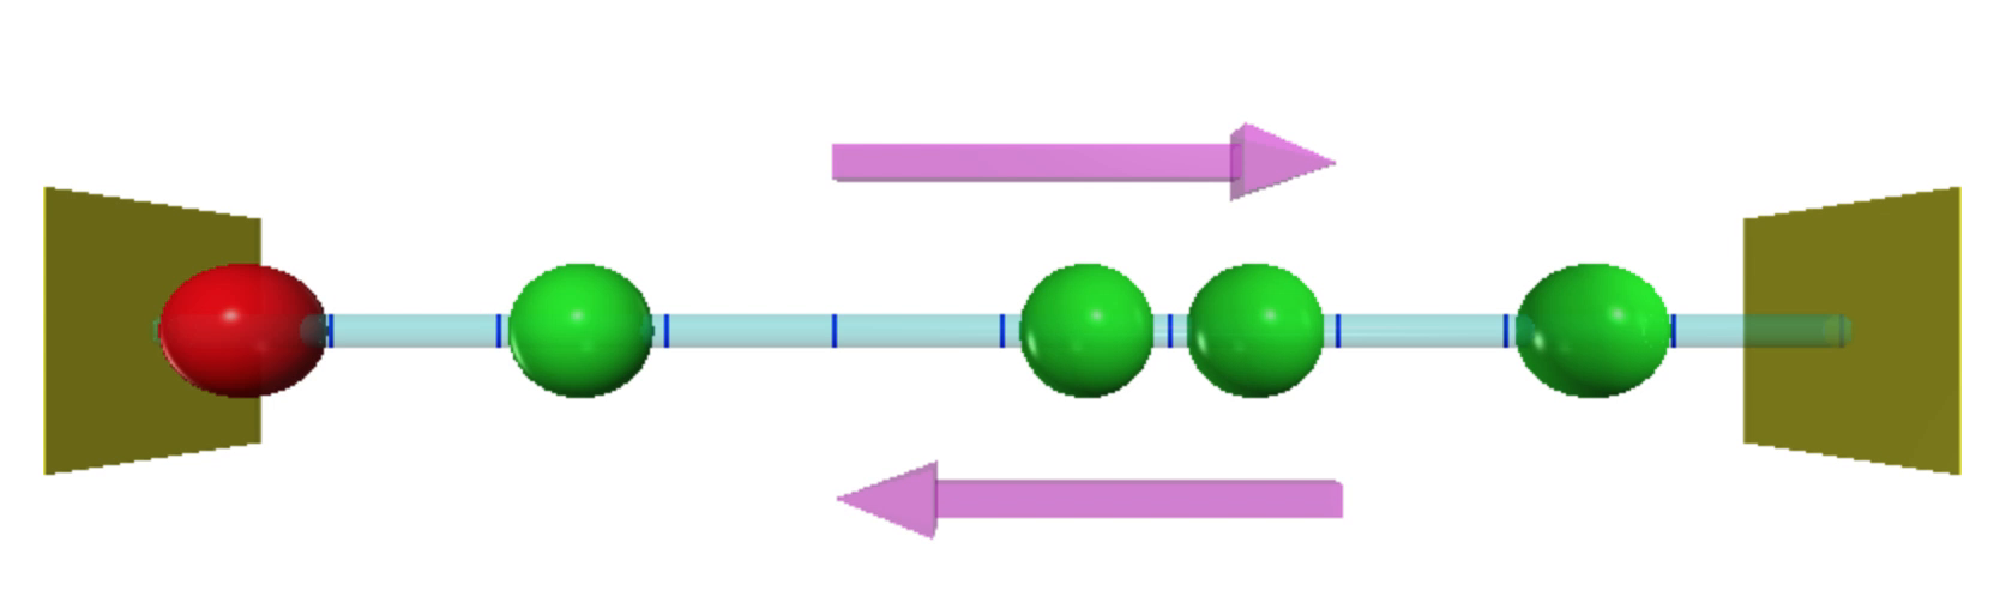
\includegraphics[width=0.8\linewidth]{betheEq}
%     \caption{Intepretation of Bethe Equation.}
%     \label{fig:betheEq}
% \end{figure}
By solving the Bethe equation, one can get $p_1$ and $p_2$ and thus all
amplitude coefficients up to a constant normalization factor. Then Eq.
\eqref{eq:eigenvaluesTwo2} gives the eigenvalues and Eq.
\eqref{eq:nonstationaryModesTwo2} gives the eigenfunctions.
Unfortunately, it might not possible to solve the Bethe equation analytically.
So we resort to numerical solutions. We have verified the resulting eigenvalues
and eigenfunctions by benchmark with the results from brute force diagonalizing
of the transition matrix for small system size $L\le10$. Notice that those roots
that $p_n=0$ or $p_n=\pi$ have to be filtered out because they correspond to the
first type of non-stationary eigenmodes which is not compatible by Eq.
\eqref{eq:nonstationaryModesTwo2}


To summarize, the complete solution of two particle hopping system with
reflecting boundaries was found. The solution is shown in the form of
eigenfunction expansion, i.e. Eq. \eqref{eq:eigenModesTwo}. The stationary
eigenfunction with eigenvalue $\Lambda_0=0$ is listed as Eq.
\eqref{eq:stationaryTwo}, while the two types of non-stationary eigenvalues and
corresponding eigenfunctions are listed in Eq. \eqref{eq:eigenvaluesTwo1},
\eqref{eq:eigenvaluesTwo2} and Eq.
\eqref{eq:nonstationaryModesTwo1}, \eqref{eq:nonstationaryModesTwo2},
respectively. They can be fully determined by  solving the Bethe Equation Eq.
\eqref{eq:betheEqTwo1} and Eq. \eqref{eq:betheEqTwo2}. Part of them are
analytically shown in Eq. \eqref{eq:eigenTwo}.

Finally, there are several remarks we want to make here.
Firstly, as one can see from Eq.  \eqref{eq:eigenTwo} that the eigenvalues of two
particle system always contain the eigenvalues of single partile system. We will
show later this can be generalised that the eigenvalues of $N+1$ particle system
always contain the eigenvalues of $N$ particle system for $N<L/2$. Secondly, the
relaxation time of the system is realted to the largest non-zero eigenvalue
$\Lambda_1$. Eq.  \eqref{eq:eigenTwo} hints
$\Lambda_1=-(\alpha+\beta)+2\sqrt{\alpha\beta} \cos\left(\frac{\pi}{L}\right)$.
However, since there is no analytical solution for eigenvalues of the second
kind, it will be difficult to rigously prove that. Nummerical evidences will be
provided to verify this is indeed true.

In next section, we will generalise the solution to the $N$ particles system.
It is actually quite straight forward after we have done the two particles
case. 


\section{General Solution of $N$ particles ASEP}
\label{sec:general_solution_of_n_particles_asep}

As before, we first write down the master equation of a $N$ particles system.
\begin{equation}
    \begin{aligned}
        \label{eq:masterEqN}
        \frac{d P(x_1, \cdots, x_N; t)}{dt} = & \sum_{j=1}^N \left[\alpha
            P(\cdots,x_j-1,\cdots;t) + \beta P(\cdots, x_j+1, \cdots;t)\right. \\ 
        & \left.- (\alpha+\beta)P(\cdots, x_j, \cdots; t)\right]
    \end{aligned}
\end{equation}

Similarly, after the eigenfunction expansion the reflecting boundaries write as
\begin{subequations}
    \label{eq:boundaries-N-particles}
    \begin{align}
        \alpha \Psi(0,x_2,\cdots,x_N) = \beta \Psi(1, x_2,\cdots, x_N) \\
        \alpha \Psi(x_1,\cdots, x_{N-1}, L) = \beta \Psi(x_1,\cdots, x_{N-1}, L+1)
    \end{align}
\end{subequations}
The exclusive condition for $N$ particles case is more tricky. In principle,
one has to consider to case of three body collision and four body collision and
so on. Luckily, in the simple model of ASEP, one can prove that these more than
two body exclusive conditions are not new but just linear recombination of two
body exclusive condition. So we can write the exclusive condition of a $N$
particles system as 
\begin{equation}
    \label{eq:exclusionConditionN}
    \alpha \Psi(\cdots,x, x,\cdots) + \beta \Psi(\cdots, x+1, x+1, \cdots) 
    = (\alpha + \beta) \Psi(\cdots, x, x+1, \cdots)
\end{equation}
The reason that the exclusive condition can be written in such a simple way is
rooting from the Yang-Baxter Equation, which encodes the integrability of the
ASEP system.

\subsection{Stationary Solution}
\label{sub:stationary_solution}

Intuitively, we construct the $N$ particles stationary solution as
\begin{equation}
    \label{eq:stationaryN}
    P^e(x_1, x_2, \cdots, x_N) = \Psi(x_1, x_2, \cdots, x_N) =  A
    \prod_{j=1}^N\left(\frac{\alpha}{\beta}\right)^{x_j}
\end{equation}

One can plug in the master equation check that the corresponding eigenvalue
$\Lambda_0= 0$, and also verify the exclusive condition as well as the reflecting
boundaries are fulfilled by insert the solution in to Eq.
\eqref{eq:exclusionConditionN} and Eq. \eqref{eq:boundaries-N-particles}
separately.

We now try to fix the parameter $A$ by normalization. Let us denote
$q:=\frac{\alpha}{\beta}$, then we can write $A$ as following
\begin{equation}
    \label{eq:stationaryPrefactor}
    A^{-1} = \sum_{\Omega} q^{\sum_j{x_j}} = 
    \sum_{x_1 < x_2 < \cdots < x_N} q^{\sum_j{x_j}}
\end{equation}
Let us do a variable change so that 
\begin{align*}
    \sum_j{x_j} &=& E_0 + E \\
    E_0 &=& 1 + 2 + \cdots + N = \frac{N(N+1)}{2}
\end{align*}
We can derive that $E$ is a integer in the range of $0, 1, \cdots, N(L-N)$. So
Eq. \eqref{eq:stationaryPrefactor} can be rewrite as 
\begin{equation}
    \label{eq:prefactorRewrite}
    A^{-1} = q^{E_0}\sum_{E=0}^{N(L-N)}g(E)q^E
\end{equation}
where $g(E)$ is the number of partitions of positive integer $E$ to $N$ parts
with each of size at most $L-N$. From the number partition theory, we identify
\begin{equation}
    \label{eq:degeneratcy}
    \sum_{E=0}^{N(L-N)}g(E)q^E = \binom{L}{N}_q =
    \frac{[L]_q!}{[L-N]_q![N]_q!}
\end{equation}
where $[N]_q = 1 + q + q^2 + \cdots + q^{N-1}$ is called a $q$ number, and Eq.
\eqref{eq:degeneratcy} is called the $q$ binomial coefficient\cite{}.
So we finally arrive at 
\begin{equation}
    \label{eq:stationarySolutionN}
    P^e(x_1, x_2, \cdots, x_N) = q^{-\frac{N(N+1)}{2}}
    \binom{L}{N}_q^{-1}\prod_{j=1}^N{q^{x_j}}
\end{equation}

In \cite{}, G. M. Sch\"{u}tz use a quantum group formalism obtained the same
result with a different notation. We emphasize here that our method is much more
easily to understand and no prerequisite knowledge of quantum mechanics and
group theory is needed.

With the equilibrium $N$ particle distribution, we can readily calculate the
equilibrium distribution of any tagged particle. Denote he distribution of the
$n$th particle $p_n(x)$, we have
\begin{equation}
    \begin{aligned}
        \label{eq:pdfTaggedParticle}
        p_n(x) = & \sum_{0<x_1<\cdots<x_{n-1}\le x-1}P^e(x_1, x_2, \cdots, x_N)
        \sum_{x<x_{n+1}<\cdots<x_{N}\le L}P^e(x_1, x_2, \cdots, x_N) \\
        = & \left. q^{(N+1-n)(x-n)} \binom{x-1}{n-1}_q\binom{L-x}{N-n}_q 
            \middle/  \binom{L}{N}_q \right.
    \end{aligned}
\end{equation}
Finally, the equilibrium density profile can be obtain by summing up $p_n(x)$
\begin{equation}
    \label{eq:densityProfile}
    \rho(x) = \sum_{n=1}^N p_n(x) 
\end{equation}


\subsection{Non-stationary Modes}
\label{sub:non_stationary_modes}

Inspired by the calculation of two particles case, we try to find the Bethe
solution of the $N$ particles system by taking the following Ansatz: 
\begin{equation}
    \label{eq:nonstationaryModesN}
    \begin{aligned}
        \Psi(x_1, x_2, \cdots, x_N) = \sum_{\sigma\in \mathcal{S}_N}
        \prod_{n=1}^N \psi_n^{\sigma}(x_{\sigma(n)})
    \end{aligned}
\end{equation}
where $\mathcal{S}_N$ is the group of permutations of $N$ elements and
$\psi_n^{\sigma}$ is the $n^{\text{th}}$ class of eigenfunction of Eq.
\eqref{eq:eigenModes}, either stationary or non-stationary. The subscript $n$
means all functions in the $n^{\text{th}}$ class share the same $p_n$, the
superscript $\sigma$ means the amplitude coefficients $A_n^{\sigma}$ or
$A_{n\pm}^{\sigma}$ are not the same for different permutations.

We again insert the solution to the master equation Eq. \eqref{eq:masterEqN},
notice that the amplitude coefficients are irrelevant with the eigenvalues. So
we obtain the simple form of corresponding eigenvalue 
\begin{equation}
    \label{eq:eigenvaluesN}
    \Lambda = \sum_{n=1}^N \lambda_n
\end{equation}
$\lambda_n$ here is a function and its expression depends on whether
$\psi_n^{\sigma}$ is stationary or non-stationary. For stationary $\lambda_n=0$,
for non-stationary $\lambda_n(p_n)=
-(\alpha+\beta)+2\sqrt{\alpha\beta}\cos(p_n)$.  Notice that, as we can see from
the two particles example, the Bethe Equations will give the value of $p_n$ and
determine the eigenvalues. In general, they are more than one solution because
Bethe Equations are nonlinear, and different solution can lead to different
eigenvalues.

We now consider that the non-stationary eigenfunctions is constructed by $N_s$ of
Eq. \eqref{eq:stationaryEigenMode} classes and $N-N_s$ of Eq.
\eqref{eq:nonstationaryEigenModes} classes. Notice that $N_s=0$ corresponds to
the second type of eigenfunctions in our discussion of the two particles system.
We will start from this case first here.

Plug Eq. \eqref{eq:nonstationaryModesN} in to the reflecting boundaries Eq.
\eqref{eq:boundaries-N-particles} we can obtain 
\begin{subequations}
    \label{eq:scatterFactorBoundaryN}
    \begin{align}
        \frac{A_{n+}^{\sigma|\sigma(1)=n}}{A_{n-}^{\sigma|\sigma(1)=n}} & = &
        -\frac{\alpha-\sqrt{\alpha\beta}
            e^{-ip_{n}}}{\alpha-\sqrt{\alpha\beta} e^{ip_{n}}}
        \\ \frac{A_{n+}^{\sigma|\sigma(N)=n}}{A_{n-}^{\sigma|\sigma(N)=n}} & = &
        -\frac{\left(\alpha-\sqrt{\alpha\beta} e^{-ip_{n}}\right)
            e^{-ip_{n}L}}{\left(\alpha-\sqrt{\alpha\beta}
                e^{ip_{n}}\right) e^{ip_{n}L}}
    \end{align}
\end{subequations}
And substitute the Ansatz in to the Exclusive condition Eq.
\eqref{eq:exclusionConditionN} we get
\begin{subequations}
    \label{eq:scatterFactorExclusiveN}
    \begin{align}
        \frac{A_{n\pm}^{\sigma}A_{(n+1)\pm}^{\sigma}}{A_{n\pm}^{\sigma|
                n\leftrightarrow n+1}A_{(n+1)\pm}^{\sigma|n\leftrightarrow n+1}}
        & = & -\frac{a(\pm p_{n},\pm p_{n+1})}{a(\pm p_{n+1}, \pm p_{n})} \\
        a(p, p^{\prime}) & = & \sqrt{\alpha\beta}e^{i(p+p^{\prime})} - (\alpha +
        \beta) e^{i p} + \sqrt{\alpha\beta}
    \end{align}
\end{subequations}
% \begin{equation}
%     \label{eq:consistencyConditionN}
%     \frac{A_{n+}^{\sigma|\sigma(1)=n}}{A_{n-}^{\sigma|\sigma(1)=n}}  
%     \frac{A_{n-}^{\sigma|\sigma(N)=n}}{A_{n+}^{\sigma|\sigma(N)=n}} = 
%     \frac{\tilde{A}_{1}\tilde{A}_{2+}}{A_{1}A_{2+}}
%     \frac{A_{1}A_{2-}}{\tilde{A}_{1}\tilde{A}_{2-}}
% \end{equation}
Then one can either use the consistency condition or the interpretation we
discussed in the two particles case and the well know periodic Bethe Equation,
easily find the following set of Bethe Equations for the $N$ particles system:
\begin{equation}
    \label{eq:betheEqN}
    e^{i2p_nL}  =  \prod_{m\neq n}^N\frac{a(p_n, p_m)}{a(p_m, p_n)} 
    \frac{a(p_m, -p_n)}{a(-p_n, p_m)}
\end{equation}
By solving Eq. \eqref{eq:betheEqN} we get all the $p_n$ and then one can plug
back in Eq. \eqref{eq:eigenvaluesN} and Eq. \eqref{eq:nonstationaryModesN} for
the corresponding eigenvalues and eigenfunctions. 

Now let us come back to the case that $0<N_s<N$. The calculation of the two
particles system is a good illustration. We can easily find out there is
nothing different except we will have only $N-N_s$ wave vectors and $2N-N_s$
amplitude coefficients. So one just have to use the relation similar to Eq.
\eqref{eq:scatterFactorExclusive} together with Eq.
\eqref{eq:scatterFactorBoundaryN} to build the Bethe Equation. Moreover, Eq.
\eqref{eq:betheEqTwo1} tells us that the Bethe Equations we can obtain will be
exact the same as the Bethe Equations of the second type $N-N_s$ particles
system. So according to Eq. \eqref{eq:eigenvaluesN} for the eigenvalues, we can
conclude that the eigenvalues of $N-N_s$ particles system are always contained
in the eigenvalue set of $N$ particle system. Notice that this is only true for
$N<L/2$. For $N>L/2$, one can easily use the particle-hole duality which shows
that the eigenvalue of $N$ particles system should be the same as $L-N$
particles system.
% \begin{figure}[htpb]
%     \centering
%     \includegraphics[width=0.8\linewidth]{spectrum}
%     \caption{Left: embeding of eigenvalues; Right: benchmark of eigenvalues from
%         Bethe Ansatz theory to directly diagonalize transition matrix, $N=2$.
%         $L=10$, $\alpha=2$ and $\beta=1$ for both. }
%     \label{fig:spectrum}
% \end{figure}

Finally, we remark that the Bethe Equations have to be solved numerically in
most cases. However, there is a small set of non-stationary eigenvalue and
eigenvectors we can obtain analytically, which correspond to the case with
just one excitation mode. The results are summarized as following:  
\begin{subequations}
    \label{eq:eigenN}
    \begin{align}
        \label{eq:partEigenvaluesN}
        \Lambda_k  = 
        -(\alpha+\beta) + 2\sqrt{\alpha\beta}\cos(\frac{k\pi}{L});
        ~k=1,2,\dots, L-1  \\
        \label{eq:eigenvectorsN}
        \Psi_k(x_1, x_2, \cdots, x_N)  =  A \sum_{n=1}^N
        \left(\frac{\alpha}{\beta}\right)^{n-1} \phi_k(x_n)\prod_{m\neq n} 
         \left(\frac{\alpha}{\beta}\right)^{x_m}
    \end{align}
\end{subequations}
Notice that the set of eigenvalue is exact the single particle spectrum, and
again $\phi_k(x)$ is exactly the single particle eigenfunction.
Fortunately, the numerical evidence shows that the most interesting
eigenmode, i.e. the slowest relaxation mode, is contained in this set. 
We will discuss it in next section. 

\section{Relaxation Time}
\label{sec:relaxation_time}

The largest non-zero eigenvalue we found and verified by numerical results is 
\begin{equation}
    \label{eq:largestEigenvalue}
    \Lambda_1 = -(\alpha+\beta) +
    2\sqrt{\alpha\beta}\cos(\frac{\pi}{L})
\end{equation}
If $L \gg 1$, we can expand the cos term, obtain 
\begin{equation}
    \label{eq:largestEigenvalueExpanded}
    \Lambda_1 = -(\sqrt{\beta}-\sqrt{\alpha})^2 -
    \frac{\sqrt{\alpha\beta}\pi^2}{L^2}
\end{equation}
And the relaxation time can be calculated as 
\begin{equation}
    \label{eq:relaxationTime}
    \tau = -\frac{1}{\Lambda_1}
\end{equation}

There are several information we can read form Eq.
\eqref{eq:largestEigenvalueExpanded} and \eqref{eq:relaxationTime}. Firstly, we
can see the scaling $\tau \approx L^2$, which means the dynamical exponent of
the system is $2$. Secondly, as we can see from Eq.
\eqref{eq:largestEigenvalueExpanded}, the bigger difference between $\alpha$
and $\beta$, the smaller relaxation time we will get. This is also consistent
as one would expect. If we map back to the polymer model, the result here can
be compared with the prediction of Rouse theory. Unlike the prediction
from Rouse theory that relaxation time does not depend on external force, we
have here that stronger external force decreases the relaxation time. This
point highlight the fundamental difference between the infinite extensible bead
spring model and the rigid bead rod model which is of course finite extensible. 

In Fig.  \ref{fig:eigenvalues} shows all the eigenvalues of a system with
lattice size $L=10$, calculated by brute force diagonalizing the transition
matrix.  Lattice The number of particles on the lattice is ranging from $1$ to
$9$. The difficult to calculate larger lattice size $L$ lies on that the
dimension grow as $\binom{L}{N}$, and if we take $N=L/2$, the dimension of the
matrix will became a extremely large number very soon. 

% \begin{figure}[htpb]
%     \centering
%     \includegraphics[width=0.8\linewidth]{eigenvalues}
%     \caption{Eigenvalues calculated by numerically diagonalize the transition
%         matrix.}
%     \label{fig:eigenvalues}
% \end{figure}

As we can see in Fig. \ref{fig:eigenvalues}
that all eigenvalues of case $N=1$ are contained in the set of
eigenvalues $N=2$, and all eigenvalues of case $N=2$ are contained in the set
of $N=3$ and so on until reach the largest set $N=L/2$. This means the
characteristic polynomial of $N=k+1$ always contains the factor of the
characteristic polynomial $N=k$. This is predict exactly by our theory. 

\section{Summary}
\label{sec:summeary}
We use the modified Bethe Ansatz methods solve the ASEP model with reflecting
boundaries.  The stationary distribution was solved exactly and the one
correspond to the relaxation time of the system was postulated. Numerical
evidence is provided for later statement.

\newpage

\appendix
\section{Derivation of the exclusion condition}
To derivate the exclusion condition, which is a little bit confusing at a first sight, we use the two particles example and then generalise to $N$ particle case.
First, let us rewrite the master equation of this two particle system:
\begin{equation}
    \begin{aligned}
        \label{eq:masterEqTwoGeneral}
    \frac{d P(x_1, x_2; t)}{dt} = & \alpha P(x_1-1,x_2;t) + \beta P(x_1+1,x_2;t) \\ 
    & + \alpha P(x_1, x_2-1; t) + \beta P(x_1, x_2+1; t)  \\ 
    & - 2(\alpha+\beta)P(x_1, x_2; t)
    \end{aligned}
\end{equation}
We assume the above equation is valid for the whole space. However, this is actually not true when the two particles are sitting on the neighboring sites. Let us now consider this special case separately, remember that $x_2 = x_1 + 1$. The master equation of this special case can be written as
\begin{equation}
    \begin{aligned}
        \label{eq:masterEqTwoNeighbor}
        \frac{d P(x_1, x_2; t)}{dt} = 
        & \alpha P(x_1-1,x_2;t) + \beta P(x_1, x_2+1; t)  \\ 
    & - (\alpha+\beta)P(x_1, x_2; t)
    \end{aligned}
\end{equation}
Now, let us do a subtraction, i.e. \eqref{eq:masterEqTwoGeneral} $-$ \eqref{eq:masterEqTwoNeighbor}, obtain
\begin{equation}
    \alpha P(x_1, x_2-1; t) + \beta P(x_1 + 1, x_2; t) = (\alpha + \beta)P(x_1, x_2; t)
\end{equation}
Let us then denote $x:=x_1$ and plug in $x_2 = x_1+1 = x+1$ in the above equation. We finally arrive at
\begin{equation}
    \label{eq:exclusionConditionTwo}
    \alpha P(x, x; t) + \beta P(x+1, x+1; t) = (\alpha + \beta)P(x, x+1; t)
\end{equation}

In summary, the sole master equation Eq. \eqref{eq:masterEqTwoGeneral} does not take into account the exclusion cases. In order to represent the exclusive setting, we assume Eq. \eqref{eq:masterEqTwoGeneral} is valid for the whole space, and then apply an additional condition on this equation like Eq. \eqref{eq:exclusionConditionTwo}. This condition is similar to the partial derivative of the PDF is the same at the collision boundary $x_1 = x_2$ in the continuous space case. 

Finally, in the similar way we can derive the exclusion condition for the cases $N>2$. However, it is not difficult to check that in cases of more than two particles, the three body collision or four body collision cases do not give out new conditions, just the linear combination of the two body collision conditions like Eq. \eqref{eq:exclusionConditionTwo}. This is fundamentally a result of Yang-Baxter Equation is satisfied for the ASEP model.




\subsection{Solution of General $N$ particles}
\label{sub:solution_of_general_n_particles}

\subsection{Relaxation Time}
\label{sub:relaxation_time}




%********************************** % Fourth Section  *************************************

\section{Relaxation Time of 3D Pinned Bead-rod Loop}
\label{sec:relaxation_time_of_3d_pinned_bead_rod_loop}


%********************************** % Fifth Section  *************************************
\section{The Single-file Diffusion}
\label{sec:the_single_file_diffusion}



%********************************** % Sixth Section  *************************************
\section{Summary}
\label{sec:summary}
